\section{Magnetic fields}

A magnetic field is a vector field that describes the physical influence of moving electric charges and magnetic materials. Moving electric charges in a magnetic field experience a force perpendicular to their velocity vector and to the magnetic flux density vector, which is described by the Lorenz force. Additionally, the effects of the magnetic field can be seen with permanent magnets which do not rely on macroscopic electrical currents. Permanent magnets attract or repel each other depending on their orientation and can pull on magnetic materials such as iron. The origin of macroscopic stationary magnetic fields are electrical currents and clusters of ordered magnetic moments of atoms. Magnetic moments of atoms are caused by orbital angular momentum and orbital angular momentum of subatomic particles which are quantum mechanical effects and cannot be described by classical physics.

A magnetic field is only one part of the more general electromagnetic field. Since special relativity we know that electric and magnetic fields can be transformed into each other by choosing a different frame of reference.

In classical physics, electromagnetism has its foundation in the four microscopic Maxwell's equations and the Lorentz force. In SI units the equations are the following.

\begin{equation*}
    \begin{aligned}[c]
        \nabla \cdot \bm{E} &= {\frac{\rho }{\varepsilon_{0}}}\\
        \nabla \times \bm{E} &= -{\frac{\partial \bm{B}}{\partial t}}\\
    \end{aligned}
    \qquad
    \begin{aligned}[c]
        \nabla \cdot \bm{B} &= 0\\
        \nabla \times \bm{B} &= \mu_0 \bm{J} + \mu_0 \varepsilon_0 {\frac{\partial \bm{E}}{\partial t}}\\
    \end{aligned}
\end{equation*}

\[\bm{F} = q\ (\bm{E} + \bm{v} \times \bm{B})\]

Maxwell's equations are a set of coupled linear partial differential equations. Therefore the sum of two solutions yields another solution and the fields can be decomposed into components of their origins.

There are two major variants of Maxwell's equations. The microscopic Maxwell equations (shown above) have universal applicability in classical physics but are unpractical for analytical calculations and extensive numerical simulations. Solids contain approximately $10^{23}$ atoms per $cm^3$ which interact with each other and the bound and free electrons in case of a metal. The macroscopic Maxwell equations define two additional auxiliary fields that describe the macroscopic behaviour by neglecting microscopic structures and phenomena like atoms and spins. Their use requires material specific parameters which have to be measured experimentally or calculated with huge numerical effort to describe the response of the material to electromagnetic fields.

\section{Magnetometer}

A magnetometer is an instrument that measures the local strength, direction or relative change of the magnetic field. Major classes of magnetometers are induction magnetometers (which measure only varying fields), rotating coil magnetometers, Hall effect magnetometers, NMR magnetometers, SQUID magnetometers, and fluxgate magnetometers.

Magnetometers have been miniaturized to the extent that they can be built into integrated circuits at very low cost in recent years. As \gls{mems} magnetic field sensor they are finding increasing use as miniaturized compasses. Compensation for temperature, hard iron, and soft iron effects are necessary for these applications.

Many smartphones contain miniaturized \gls{mems} magnetometers which are as compasses. The iPhone 3GS included the AN-203 produced by Honeywell, a magnetoresistive permalloy sensor.\cite{magnetometer_1} In 2009, the price of three-axis magnetometers dipped below one US dollar per device and dropped rapidly. Hall effect devices are also popular.\cite{magnetometer_2}

\subsection{Hall-effect sensor}

\begin{figure}[h]
    \centering
    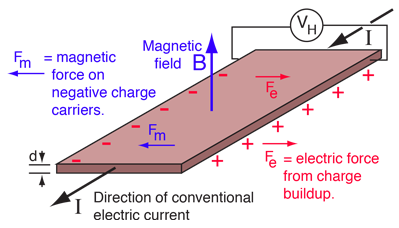
\includegraphics[width=0.5\textwidth]{figures/hall_effect.png}
    \caption{Schematic of a Hall probe measuring the magnetic field.}
    \label{fig:hall_effect}
\end{figure}

The Hall-effect can be used to measure the magnitude of magnetic fields in one direction and is called after Edwin Hall who discovered it in 1879.

The effect is illustrated in Figure \ref{fig:hall_effect}. Magnetic fields exert a transverse force on moving charge carriers. This includes electrical currents in conductors. There the magnetic field is pushing the charges to one side of the material which is most evident in a thin flat conductor. The imbalance of the charges results in a measurable voltage between the two sides of the conductor. Its output voltage is directly proportional to the passing magnetic field strength.

\[V_H = \frac{I B}{n e d}\]

With $I$ as the current flowing through the probe, $B$ the magnetic field perpendicular to the probe, $n$ as the charge carrier density, $e$ the elementary charge, and the probe thickness $d$.

\section{Earth's magnetic field}

The Earth is sourcing a magnetic field from its interior which is reaching out into space, where it interacts with charged particles emitted by the Sun (streams of these particles are called solar wind). The magnetic field is believed to be generated by electric currents in conductive convection streams of molten iron and nickel due to heat escaping the Earth's core. This process in very complex and an active field of research. The magnitude of the magnetic flux density ranges from $25$ to $65\ \mu T$. The field can be approximated by a magnetic dipole tilted at an angle of about $11$ degrees with respect to Earth's rotational axis.

At any location, the Earth's magnetic field can be represented by a three-dimensional vector. A typical procedure for measuring its direction is to use a compass to determine the direction of magnetic North. Its angle relative to true North is the declination or variation. Facing magnetic North, the angle the field makes with the horizontal is the inclination or magnetic dip. The intensity of the field is proportional to the force it exerts on a magnet. Another common representation is in X (North), Y (East) and Z (Down) coordinates.\cite{earth_magnetic}

\begin{figure}[hbt!]
    \centering
    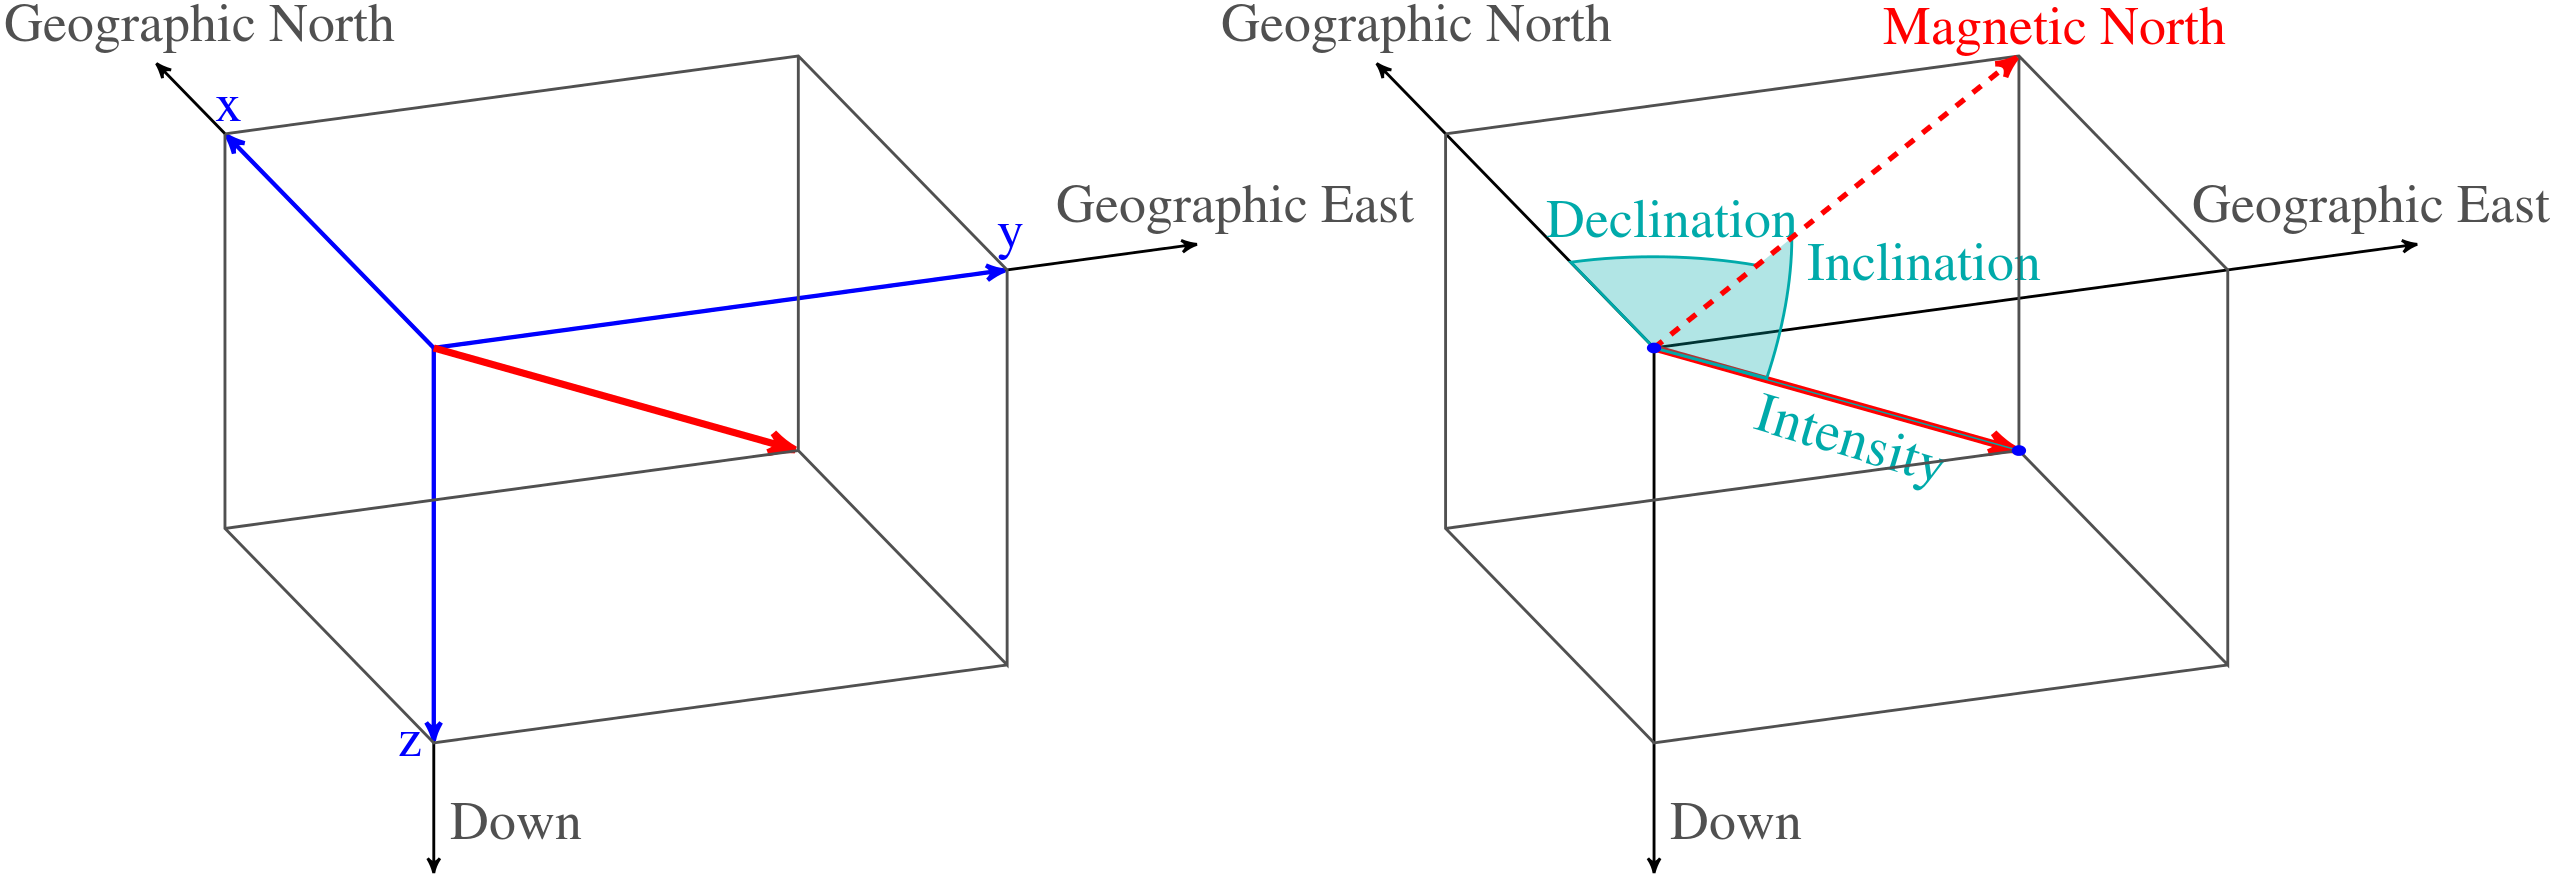
\includegraphics[width=1.0\textwidth]{figures/earth_magnetic_field_coords.png}
    \caption{Common coordinate systems used for representing the Earth's magnetic field.}
    \label{fig:earth_magnetic_field_coords}
\end{figure}

\subsection{Dipole approximation}

In close proximity to the surface of the Earth, its magnetic field can be approximated by the field of a magnetic dipole placed at the center of the Earth and oriented with an angle of about $11^{\circ}$ to the rotational axis of the Earth. In this description the Earth can be viewed as a powerful bar magnet with its south pole pointing towards the geomagnetic North Pole. The dipolar field accounts for approximatly $80-90\%$ of the field in most locations.\cite{earth_magnetic}

The dipole magnetic field of the Earth can be described as follows.\cite{earth_dipole}

\[\bm{B}_r = -2 \bm{B}_0 ({\frac{R_E}{r}})^3 \cos \theta\]
\[\bm{B}_\theta = - \bm{B}_0 ({\frac{R_E}{r}})^3 \sin \theta\]

With $B_0$ as the mean value of the magnetic flux density at the magnetic equator on the Earth's surface. Typically $B_0 = 3.12*10^{-5}\ \textrm{T}$. $R_E$ is the mean radius of the Earth (approximately $6370\ \textrm{km}$), $r$ is the radial distance from the center of the Earth, and $\theta$ is the azimuth angle measured from the north geomagnetic pole.

This approximation is very practical for our purposes since it is easy to calculate the magnetic flux density for a given WGS84 position.

\section{Quaternions}

Quaternions are a number system that extends the complex numbers with two additional imaginary axis. In 1843, they were described by the Irish mathematician William Rowan Hamilton and applied to mechanics in three-dimensional space.

Quaternions are generally represented in the form:

\[a + b \bm{i} + c \bm{j} + d \bm{k}\]

where $a$, $b$, $c$, and $d$ are real numbers, and $\bm{i}$, $\bm{j}$, and $\bm{k}$ are the fundamental quaternion units (similar to the imaginary unit $\bm{i}$).

The imaginary units are connected through multiplication as follows

\[\bm{i}^2 = \bm{j}^2 = \bm{k}^2 = \bm{ijk} = -1 \textrm{.}\]

Quaternions are used in theoretical mathematics and applied mathematics. Applications are calculations involving three-dimensional rotations such as in computer graphics, computer vision, and crystallographic texture analysis. In practical applications, they can be used alongside other methods, such as Euler angles and rotation matrices, or as an alternative to them.

The unit quaternions can be thought of as a choice of a group structure on the 3-sphere $S^3$ that gives the group $Spin(3)$, which is isomorphic to $SU(2)$ and also to the universal cover of $SO(3)$.

The conjugate of $q$ is given by $q^* = a - b \bm{i} - c \bm{j} - d \bm{k}$.

The norm by $\lVert q\rVert = \sqrt{qq^*} = \sqrt{q^{*}q} = \sqrt{a^2 + b^2 + c^2 + d^2}$.

The inverse by $q^{-1} = \frac{q^*}{\lVert q\rVert ^2}$.

\subsection{Quaternions as rotations}
% mention that a quaternion can be constructed from euler axis+angle?
% mention that all rotations in 3D can be parameterized as euler axis+angle and therefore as quaternion?

To express a rotation of an angle $\theta$ around a unit vector $\bm{u} = u_x \bm{i} + u_y \bm{j} + u_z \bm{k}$ we compose a unit quaternion with the extended Euler's formula

\[\bm{q} = e^{{\frac{\theta}{2}}{\bm{u}}} = \cos{\frac{\theta}{2}} + \sin{\frac{\theta}{2} \bm{u}} \textrm{.}\]

In order to apply this rotation to a point $\bm{p} = p_x \bm{i} + p_y \bm{j} + p_z \bm{k}$ one has to compute

\[\bm{p}' = \bm{q} \bm{p} \bm{q}^{-1} \textrm{.}\]

Rotations can be composed by multiplying quaternions and reversed by the inverse quaternion $\bm{q}^{-1}$.

\begin{figure}[hbt!]
    \centering
    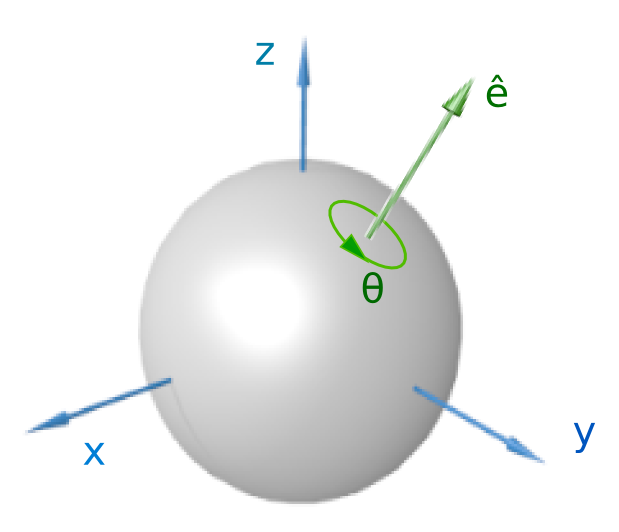
\includegraphics[width=0.5\textwidth]{figures/quaternion_rot.png}
    \caption{A visualization of a rotation represented by an Euler axis and angle.}
    \label{fig:quaternion_rot}
\end{figure}

\section{Bayesian statistics}

Bayesian statistics is a theory based on the Bayesian interpretation of probability where it expresses a degree of belief in an event. The degree of belief may be based on prior knowledge about the event, such as the results of previous experiments, or on personal beliefs about the event. This differs from the frequentist interpretation that views probability as the limit of the relative frequency of an event after many trials.\cite{bayes_1}

Bayes' theorem is a fundamental theorem in Bayesian statistics which is used by Bayesian methods to update probabilities after obtaining new data. Given two events $A$ and $B$, the conditional probability $P(A\ |\ B)$ -- the probability for $A$ given that $B$ is true -- is expressed as follows:

\begin{equation}
\label{eq:bayes}
    P(A\ |\ B) = \frac{P(B\ |\ A) P(A)}{P(B)} \ \ \textrm{with} \ \ P(B) \ne 0
\end{equation}

Although Bayes' theorem is a fundamental result of probability theory, it has a specific interpretation in Bayesian statistics. In \ref{eq:bayes}, $A$ usually represents a proposition (prior information, such as the statement that a coin lands on heads fifty percent of the time) and $B$ represents the evidence, or new data that is to be taken into account (such as the result of a series of coin flips). $P(A)$ is the prior probability of $A$ which expresses one's beliefs about $A$ before evidence is taken into account. The prior probability may also quantify prior knowledge or information about $A$. $P(B\ |\ A)$ is the likelihood function, which can be interpreted as the probability of the evidence $B$ given that $A$ is true. The likelihood quantifies the extent to which the evidence $B$ supports the proposition $A$. $P(A\ |\ B)$ is the posterior probability -- the probability of $A$ after taking the evidence $B$ into account. Essentially, Bayes' theorem updates one's prior beliefs $P(A)$ after considering the new evidence $B$.\cite{bayes_1}
